\section{Implementation}\label{sec:implementation}

To implement \sysname{}, we use the basic match-action functionality that is
available in most modern commodity switches. However, correct implementation
requires a key insight into the way PFC PAUSE frames are handled.

\begin{figure}
	\hspace{-0.2in}
	\centering
	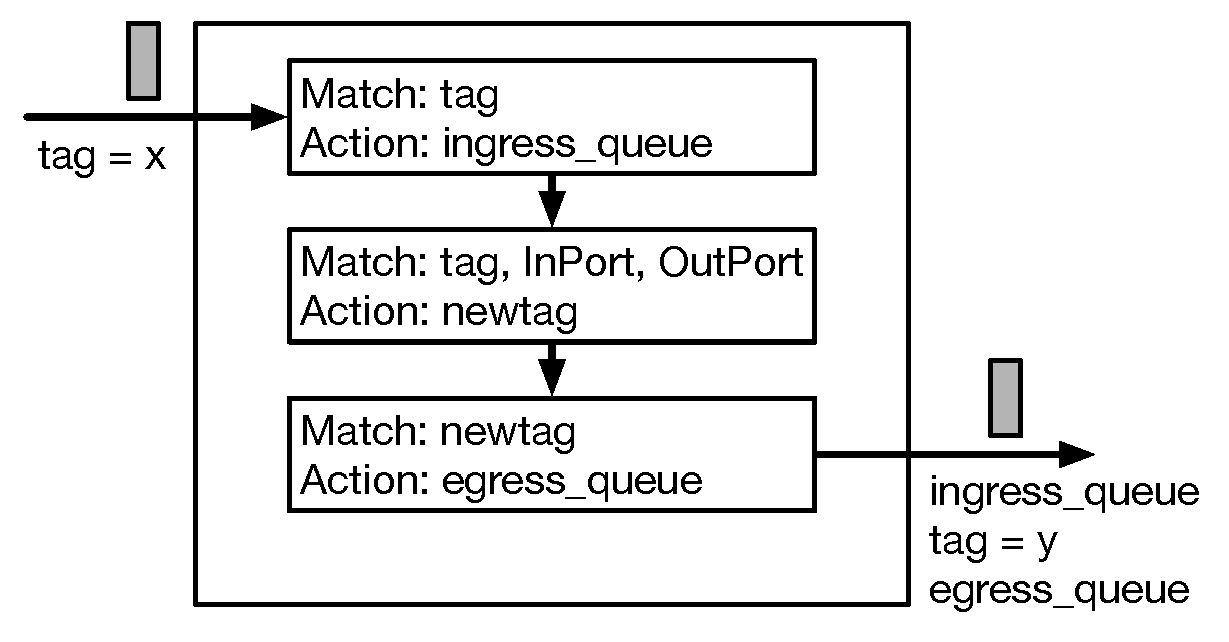
\includegraphics[width=0.5\textwidth] {figs/Tagger}
	\caption{Tagger match-action rules}\label{fig:tagger}
	
\end{figure}

\para {Math-Action rules:} \sysname{} needs to perform two operations at every
hop in the network, i.e., {\em tag-based priority queueing} and {\em tag
rewriting}.  These two operations are implemented using a 3-step match-action
pipelines shown in Figure~\ref{fig:tagger}.  In the first step, \sysname{}
classifies packets into ingress queues based on the value of tags. In the second
step, \sysname{} rewrites the value of tag based on (tag, inport, outport)
information. These two steps form the core of \sysname{}.
 
\begin{figure}[t]
 	\centering
 	\subfloat[short for lof][Ingress priority = egress priority  $\rightarrow$ packet drop.] {
 		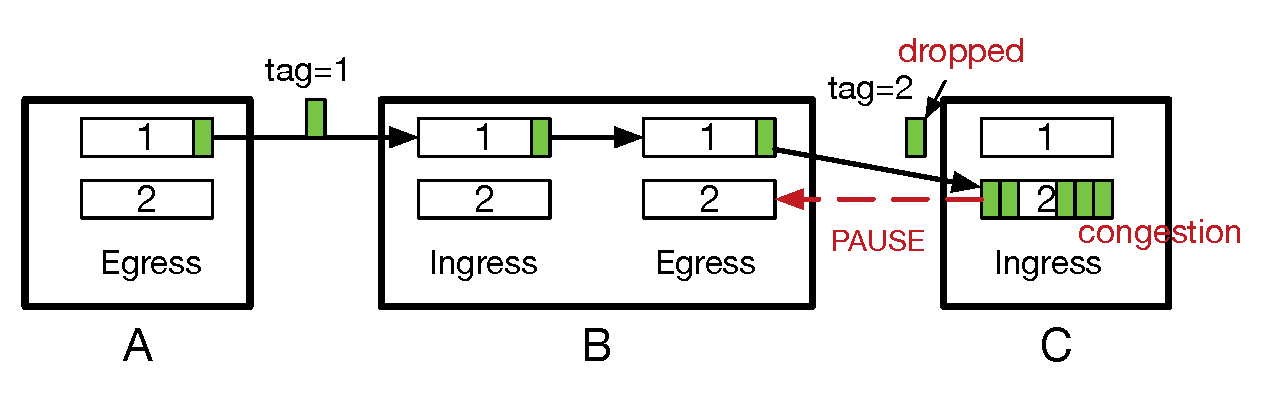
\includegraphics[width=0.43\textwidth] {figs/prioritydecoupling_1}
 	}

 	\subfloat[short for lof][Ingress priority = 1, egress priority = 2 $\rightarrow$ no drop.]{
 		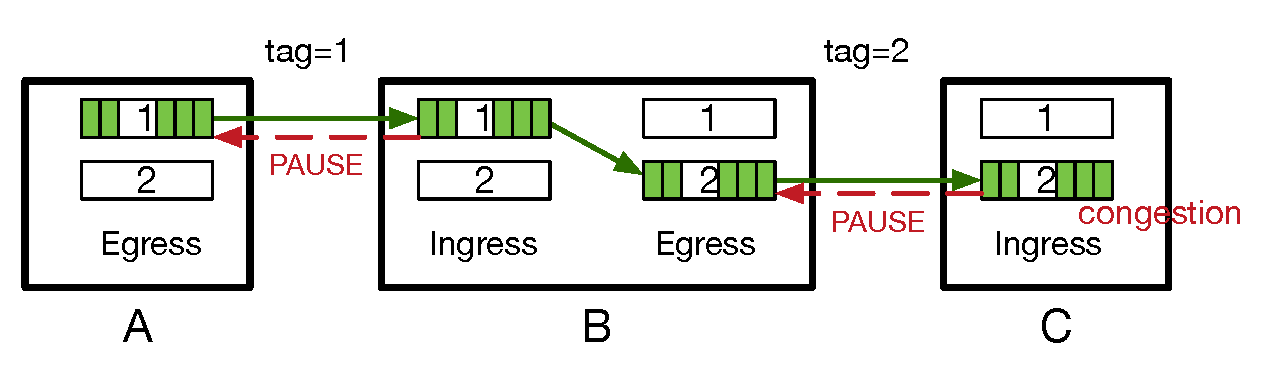
\includegraphics[width=0.43\textwidth] {figs/prioritydecoupling_2}
 	}
 	\caption{Decoupling ingress priority from egress priority at switch B is necessary for ensuring lossless priority transition.}\label{fig:prioritydecoupling}
\end{figure}

\para{Handling priority transition:}
{\em The third step, wherein the packet is placed in an egress queue based on the
{\em new} tag value, is needed to ensure correct PFC operation when priority
values are rewritten.}

Note that the tagged graph $G$ only defines the mapping between tags and ingress
queues. By default, a switch will enqueue a departing packet in the egress queue
of the same priority class as its ingress queue. This default behavior can lead
to packet loss when priority transition is performed. An example is shown in
Figure~\ref{fig:prioritydecoupling}. 
 
In this example, switch B is configured to do priority transition for packets
received from switch A and destined for switch C. It is important to note that
in this diagram, only {\em one port} on each switch is active. The two queues
are for two priorities.
 
In Figure~\ref{fig:prioritydecoupling}(a), we consider the default behavior.
Packets exit egress queue 1 at switch B, but with priority 2.  This can lead to
to packet loss when ingress queue 2 of switch C becomes congested, because 
the PFC PAUSE from switch C to switch B carries priority 2, and cannot pause 
the offending egress queue 1 of switch B. 
 
In Figure~\ref{fig:prioritydecoupling}(b), we map the packet to the egress queue
based on its new priority.  This avoids packet loss, since the PFC from switch C
correctly pauses the queue on which the packet with the new tag would be
exiting. This example thus demonstrates the necessity of the third step.

\para{Rule compression with bit masking technique:}  The match-action rules of \sysname{} can be implemented with TCAM. Entries in TCAM are bit masking based and consist of three parts ({\em Value}, {\em Mask}, {\em Result}). {\em Value} refers to the pattern to be matched, {\em Mask} refers to the mask bits associated with the pattern and {\em Result} refers to the action that occurs when a lookup hits the pattern. For example, (Value = 1000$_{(2)}$, Mask = 1100$_{(2)}$, Result = Deny) can match pattern ``$10**$'' and perform {\em Deny} action. One TCAM entry can have several Value-Mask pairs to match multiple packet header fields simultaneously, e.g., we can configure a TCAM entry like (Value-1, Mask-1, Value-2, Mask-2, Result) to match two fields simultaneously.

\begin{figure}
	\centering
	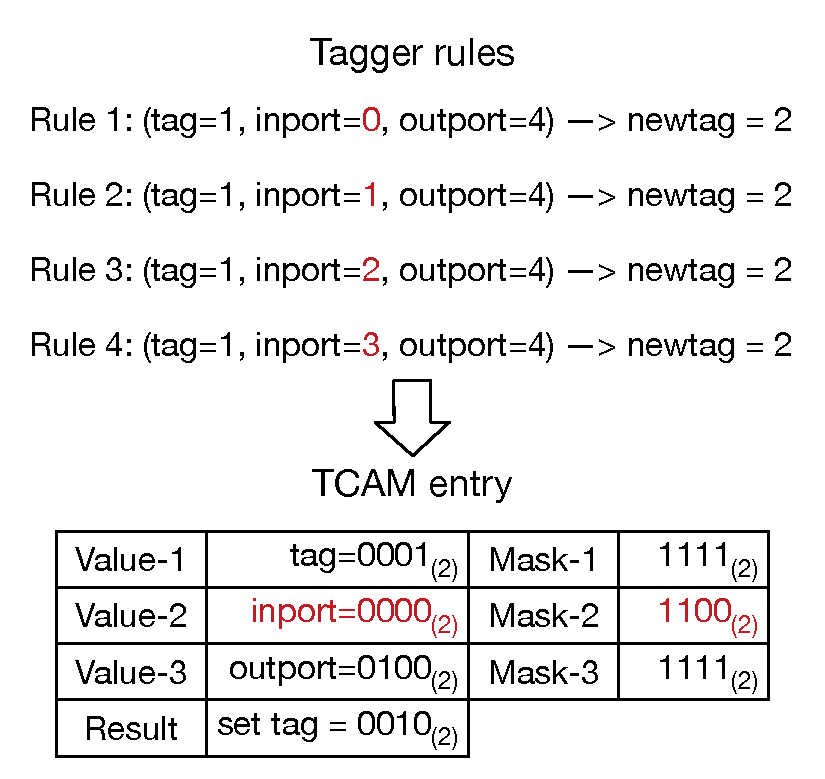
\includegraphics[width=0.45\textwidth] {figs/compression_with_bitmasking}
	\caption{An example to show rule compression with bit masking.}\label{fig:compression}
	
\end{figure}


Bit masking feature of TCAM can be leveraged to do rule compression. Rules that have the same action can be compressed into one TCAM entry, if the patterns to be matched can be aggregated using bit masking. An example is shown in Figure~\ref{fig:compression}. 

As we can see, these three rules share the same tag value, egress port and tag rewriting action. Note that most commodity switches internally use the format of port bitmap for port matching. Hence we can aggregate all the ingress ports to be matched with a value that sets all the corresponding bits to be ``1'', as shown in Figure~\ref{fig:compression}(colored as red). The observation here is that we can always aggregate the ingress ports for rules share the same tag value, egress port and tag rewriting action.

As discussed in Section~\ref{sec:generic}, without any compression, we will need $n(n-1)\times \frac{m(m-1)}{2}$ rules per switch. The number of rules can be compressed to $n\times \frac{m(m-1)}{2}$ by aggregating ingress ports. Note that the result may be further improved by doing aggregation on tag, ingress port and egress port together. 

%But $n\times m$ is already good enough as modern commodity switches typically have less than 100 ports, but can support 1-4K
%TCAM based ACL rules~\cite{xx}.

\para{Broadcom implementation:}
We have implemented \sysname{} on commodity switches based on Broadcom chipsets.
We use DSCP field in IP header as the tag. DSCP rewriting is supported by most
commodity chipsets available in the market today. DSCP-based priority queuing
(step 1) is supported natively by all switch ASIC vendors. We implement step 2
using ingress ACL rules that map (DSCP, inport, outport) to new DSCP. 

Step 3 is similarly implemented using ACLs, although the implementation requires
keen understanding how packets progress through the match-action pipeline. We
omit these gritty details for brevity. While the implementation of this step is
Broadcom-specific, we believe that ASICs from other vendors can also support
this functionality.

We stress that none of the three steps require any changes to the switch ASIC,
and everything is implemented using publicly available and documented
functionality.

\begin{figure}[t]
	%\vspace{-0.1in}
	\centering
	
	\subfloat[short for lof][Experiment scenario.]{
		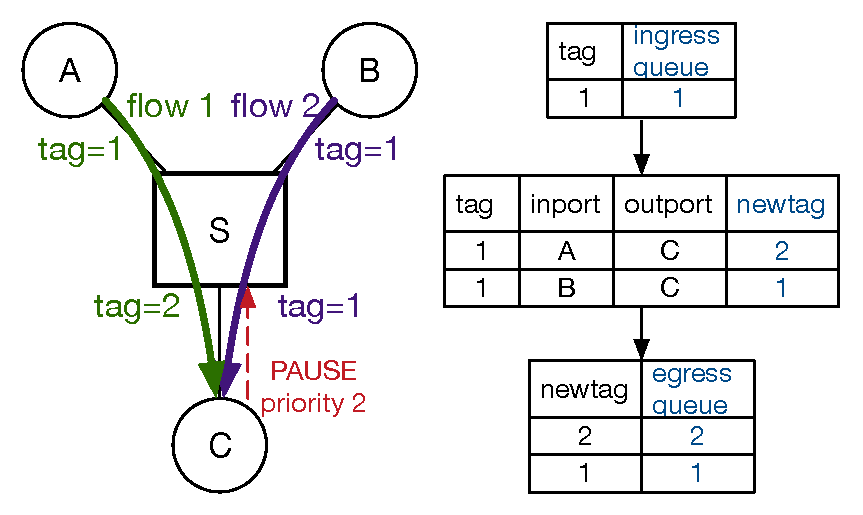
\includegraphics[width=0.25\textwidth] {figs/demon_scenario}
	}
	\subfloat[short for lof][Rate of flow 1 and flow 2.]{
	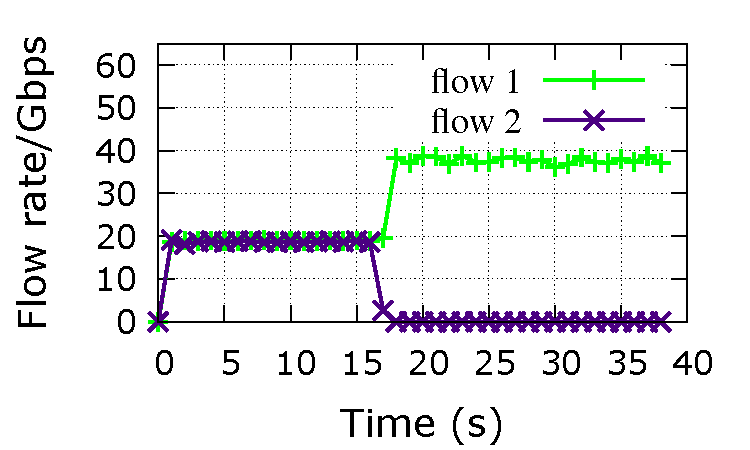
\includegraphics[width=0.25\textwidth] {figs/demon_flowrate}
}
	
	\caption{The match-action rules in action}\label{fig:tagger_demon}
\end{figure}


\para{Simple demonstration:}  A simple experiment shown in
Figure~\ref{fig:tagger_demon} demonstrates the behavior of the match-action
rules.  We generate two flows, flow 1 and flow 2, to send packets to C from
different servers connected to ports A and B. Both servers set the DSCP value in
outgoing packets to 1. The match-action rules are set to rewrite the tag value
of packets arriving on port A to 2, and forward them to port C. Tag of packets
arriving on port B is not changed.
 
At time = 17s, C sends a stream of forged PFC PAUSE frames on priority 2 to
switch S. The rate of both flows is plotted in Figure~\ref{fig:tagger_demon}(b)
(link capacity = 40Gbps). As expected, after priority 2 is paused, rate of
flow 1 is reduced to 0 while flow 2 gets all the available bandwidth. 
Counters on switch S further confirm that no packets were dropped, and server
connected to port A was paused as expected.
